\section*{Sistemas de Propulsión y Motores de Combustión}

\begin{center}
	\begin{tikzpicture}
		\node[inner sep=0pt, rounded corners=10pt] (myimage)
		{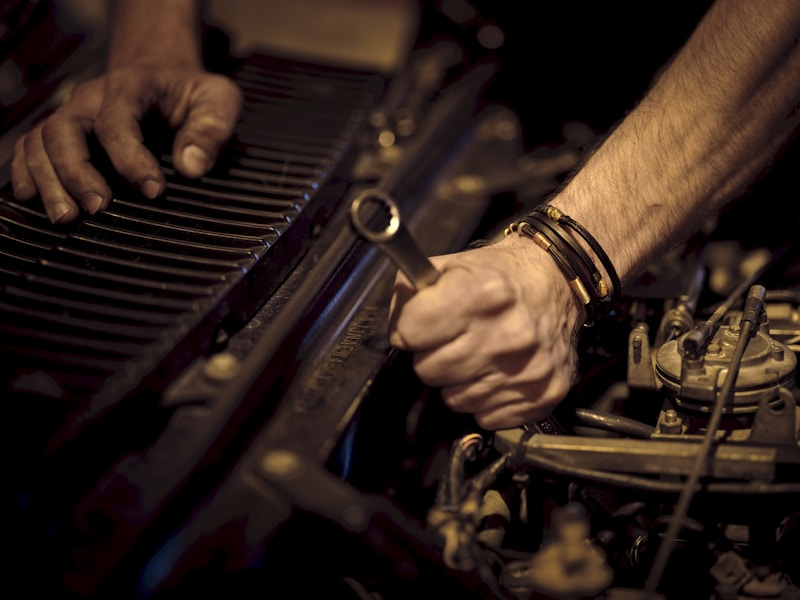
\includegraphics[width=0.6\textwidth,height=6cm]{img/cap2_motor.jpg}};
	\end{tikzpicture}
\end{center}

El motor de combustión interna, particularmente el motor Diesel, representa el corazón
energético de la maquinaria agrícola. Su función principal es transformar la energía
química contenida en el combustible en energía mecánica utilizable para tracción y
accionamiento de implementos. Comprender su funcionamiento es fundamental para un
mantenimiento que garantice potencia, eficiencia y una larga vida útil.

\subsection*{Fundamentos del Ciclo Diesel}
A diferencia de los motores de encendido por chispa, el motor Diesel utiliza el
calor generado por la alta compresión del aire en la cámara de combustión para
ignorar el combustible inyectado. Este ciclo, compuesto por las fases de admisión,
compresión, combustión/expansión y escape, requiere un control preciso de la
mezcla aire-combustible y de la temperatura operativa para maximizar el rendimiento.

\subsection*{Sistemas Auxiliares}
Para garantizar una operación eficiente, el motor depende de sistemas críticos:
\begin{itemize}
	\item \textbf{Sistema de Lubricación:} Reduce la fricción y disipa el calor en
	      partes móviles (pistones, cigüeñal, árbol de levas).
	\item \textbf{Sistema de Refrigeración:} Mantiene la temperatura dentro de los
	      rangos óptimos de trabajo, evitando deformaciones por dilatación térmica.
	\item \textbf{Sistema de Alimentación y Filtrado:} Asegura el suministro de
	      combustible y aire limpios, vital para prevenir el desgaste prematuro de
	      bombas e inyectores.
\end{itemize}

\section*{\faPencil\space Investigar y responder}
\begin{enumerate}
	\item Explique detalladamente la diferencia técnica entre el ciclo de trabajo de
	      un motor Diesel y un motor naftero (Otto).
	\item ¿Cuál es la función específica del termostato en el sistema de
	      refrigeración y qué consecuencias implica su mal funcionamiento?
	\item Describa la importancia de la viscosidad del aceite lubricante y cómo
	      afecta el desempeño del motor en climas extremos.
	\item ¿Qué papel juega el turbocompresor en el aumento de potencia de los motores
	      agrícolas modernos?
	\item ¿Qué indica la presencia de humo negro, azul o blanco por el escape de un
	      tractor Diesel?
	\item Explique qué es la relación de compresión y por qué es superior en los
	      motores Diesel.
	\item ¿Cuál es la función del sistema de filtrado de combustible y por qué el
	      agua es un contaminante crítico?
	\item Investigue los efectos de la sobrecarga operativa en la vida útil de los
	      componentes del tren alternativo del motor.
\end{enumerate}

\section*{\faWrench\space Resolver los siguientes problemas}
\begin{enumerate}
	\item Dado un manual de mantenimiento, identifique el intervalo de cambio de
	      aceite y filtros para un motor de 150 HP y justifique si debe acortarse en
	      condiciones de alta polución.
	\item Un tractor presenta dificultades de arranque en frío. Proponga una
	      secuencia de diagnóstico para el sistema de alimentación y precalentamiento.
	\item Calcule el volumen de refrigerante necesario para un sistema cuya capacidad
	      total es de 20 litros, considerando una mezcla recomendada de 50/50.
	\item Analice el desgaste prematuro de un conjunto camisa-pistón. ¿Qué pruebas
	      realizaría para determinar si la causa es lubricación deficiente o
	      filtración de aire?
	\item Diseñe una hoja de registro para el seguimiento del consumo de aceite
	      lubricante entre servicios, incluyendo el horómetro de la máquina.
	\item Ante una pérdida de potencia notable, ¿cómo realizaría una prueba de
	      estanqueidad de cilindros?
	\item Describa el procedimiento paso a paso para purgar aire del sistema de
	      combustible en un motor Diesel tras un cambio de filtros.
	\item Si la temperatura de operación supera los 100°C, enumere los componentes
	      críticos a inspeccionar (radiador, bomba, sensores).
	\item Calcule el consumo horario de combustible de un tractor que operó 8 horas y
	      requirió 120 litros para rellenar el tanque al máximo.
	\item Investigue y explique el proceso de regulación de luz de válvulas en un
	      motor agrícola convencional.
\end{enumerate}
